\chapter{Проектирование и реализация нейронной сети для решения задачи регрессии для нахождения энергии основного состояния молекулы языке Python с использованием библиотек Keras и TensorFlow}
Целью данной работы является проектирование, реализация и обучение модели нейронной сети решающей задачу регрессии для нахождения энергии основного состояния квантово-механической системы. Для достижения цели был использован язык Python, библиотеки Keras и Tensorflow.
\section{Поиск и подготовка данных для обучения}
Поиск данных для обучения производился в системе организации конкурсов по исследованию данных kaggle. Он содержит множество наборов данных для совершенно различных задач. Для данной работы был выбран набор Predict Molecular Properties. Он содержит данные о структуре 250000 молекул взятые с базы данных PubChem и представленные в формате json, эти данные в ходе работы были разбиты на 3 части:
\begin{enumerate}
    \item [1)] выборка для обучения, содержащая данные о 100000 молекул;
    \item [2)] выборка валидации, содержащая данные о 50000 молекул;
    \item [3)] тестовая выборка, содержащая данные о 100000 молекул.
\end{enumerate}


\newpage


\section{Реализация модели на языке Python и обучение сети}
Для напсиания программы были использованы библиотеки Keras и Tensorflow. Класс Sequential представляет собой линейный стек слоев. С помощью него можно достаточно просто создать необходимую модель. Он автоматически настраивает все связи между слоями, а также добавляет нейроны смещения. В листинге \ref{ls:1} во входных параметрах передаются 5 слоев:
\begin{enumerate} 
  \item[1)] входной слой класса Dense, состоящий из 1000 нейронов, который принимает на вход вектор признаков состоящий из 1275 элементов, с функцией активации ReLu;
  \item[2)] скрытый слой класса Dense, состоящий из 500 нейронов с функцией активации ReLu;
  \item[3)] скрытый слой класса Dense, состоящий из 50 нейронов с линейной функцией активации;
  \item[4)] выходной слой класса Dense, в котором 1 нейрон с линейной функцией активации;
\end{enumerate}

\begin{lstlisting}[caption={Описание модели нейросети},language=python, label={ls:1}]
model = Sequential([Dense(1000, input_dim=(1275), activation='relu'),
                        Dense(500, activation='relu'),
                        Dense(50, activation='linear'),
                        Dense(1)])
\end{lstlisting}

В листинге \ref{ls:2} указан метод для настройки процесса обучения:

\begin{lstlisting}[caption={Использовние метода compile()},language=python,label={ls:2}]
self.classifier.compile(
    optimizer='adam', 
    loss='mean_squared_error'
)
\end{lstlisting}
Метод compile() на вход принимает 2 параметра:
\begin{enumerate} 
  \item[1)] метод оптимизации алгоритма градиентного спуска. Для данной модели был выбран метод Adam;
  \item[2)] функция ошибки (потерь), он же критерий качества, который программа будет использовать для корректировки весов во время обратного распространения ошибки. Для задач регрессии отлично подходит критейрий качества средний квадрат ошибки \ref{e:9}:
\begin{equation} \label{e:9}
 E = \frac{1}{N}\sum (t_{i}-y_{i})^2.
\end{equation}
\end{enumerate}

В листинге \ref{ls:3} указан метод get\_data, который считывает данные из csv-файлов и возвращает в виде массива numpy.
\begin{lstlisting}[caption={Определение метода get\_data},language=python,label={ls:3}]
def get_data(path):
    data = pd.read_csv(path + "train/molecules.csv")
    df = data.drop(['Unnamed: 0', 'pubchem_id'], axis=1)
    df = df[(df.T != 0).any()]
    X = df.drop(['En'], axis=1)
    Y = df['En']
    y_train = Y.values
    x_train = X.values

    data = pd.read_csv(path + "test/molecules.csv")
    df = data.drop(['Unnamed: 0', 'pubchem_id'], axis=1)
    df = df[(df.T != 0).any()]
    X = df.drop(['En'], axis=1)
    Y = df['En']
    y_test = Y.values
    x_test = X.values

    data = pd.read_csv(path + "val/molecules.csv")
    df = data.drop(['Unnamed: 0', 'pubchem_id'], axis=1)
    df = df[(df.T != 0).any()]
    X = df.drop(['En'], axis=1)
    Y = df['En']
    y_val = Y.values
    x_val = X.values
    return x_train, y_train, x_test, y_test, x_val, y_val
\end{lstlisting}

В листинге \ref{ls:4} запускается процесс обучения с помощью метода fit() и сохраняются обученные значения весов в файл weights.h5 методом save\_weights():
\begin{lstlisting}[caption={Использовние метода fit() и save\_weights()},language=python,label={ls:4}] 
history = model.fit(x_train,
                        y_train,
                        validation_data=(x_val, y_val),
                        callbacks=[monitor],
                        epochs=epochs,
                        batch_size=50)
model.save_weights('weights.h5')
\end{lstlisting}

На рисунке \ref{fig:5} изображены графики зависимости точности и ошибок на учебном наборе и на выборке валидации от эпохи обучения. Справедлио заметить, что на выборке валидации процент ошибок после 37 эпохи становится больше, чем на наборе для обучения. Это означает, что алгоритм начинает переобучаться после 37 эпохи. В таком случае стоит остановиться на 37 эпохе обучения и сохранить веса.
\begin{figure}[!h] 
  \center
  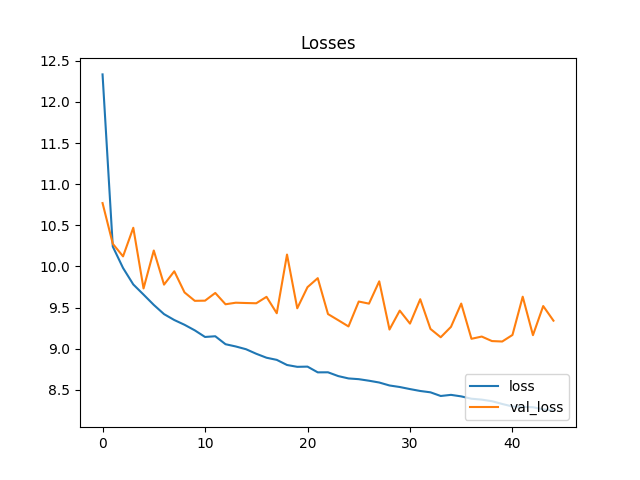
\includegraphics [scale=0.9] {img/losses.png}
  \caption{Графики зависимости ошибки нейронной сети от эпохи обучения} 
  \label{fig:5}  
\end{figure}

Сохранив веса, можно начать проверку точности на тестовой выборке. На рисунке \ref{fig:6} указан график прогноза на произвольные 200 молекул. 
\begin{figure}[!h] 
  \center
  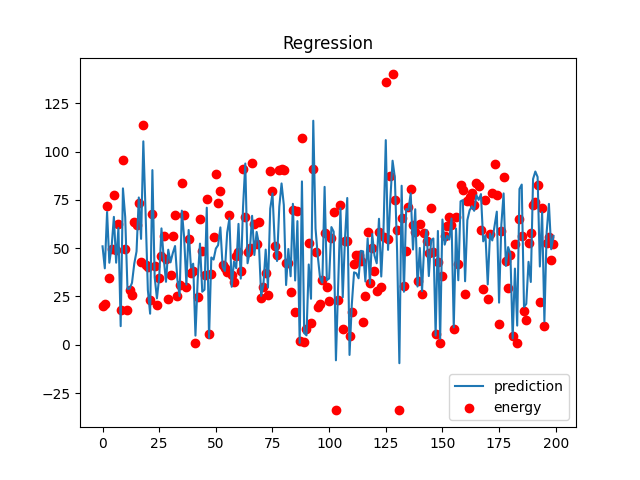
\includegraphics [scale=0.9] {img/regression.png}
  \caption{Данные тестовой выборки (отмечены красным) и функция прогноза программы (отмечена синим)} 
  \label{fig:6}  
\end{figure}
\section{Тестирование качества работы нейронной сети}
Для оценки качества работы сети нужно посчитать метрики качества работы сети. Их будет 3:

\begin{enumerate}
    \item [1)] среднеквадратичное отклонение, root mean squared error(RMSE), он рассчитывается по формуле \ref{e:10}:
    \begin{equation} \label{e:10}
        RMSE = \sqrt{\frac{1}{N}\sum (d_{n}-y_{n})^2},
    \end{equation} 
    где $d_n$ — предсказание нейросети, $y_n$ — значение энергии молекулы из тестовой выборки, N — количество элементов в тестовой выборке;
    \item [2)] средний модуль отклонений, mean absolute error(MAE), который расчитывается по формуле \ref{e:11}:
    \begin{equation} \label{e:11}
        MAE = \frac{1}{N}\sum |d_{n}-y_{n}|,
    \end{equation}
    \item [3)] средний абсолютный процент ошибки, mean absolute percentage error(MAPE), который считается по формуле \ref{e:12}:
    \begin{equation} \label{e:12}
        MAPE = 100\% \cdot \frac{1}{N}\sum \frac{|d_{n}-y_{n}|}{max(|Y|, \epsilon)},
        где \epsilon — малое число, которое используется для избежания деления на 0.
    \end{equation}
\end{enumerate}
В листинге \ref{ls:5} указан вывод программы после расчета вышеуказанных характеристик. Энергия в базе данных была выражена в ккал/моль, соответственно среднее отклонение (MAE) не превышает 10 ккал/моль, а среднеквадратичная ошибка (RMSE) не более 15 ккал/моль, что является неплохим показателем учитывая распределение энергий (рисунок \ref{fig:7}). Средний процент отклонения (MAPE) составил всего около 3.5\%.   
\begin{lstlisting}[caption={Посчитанные значения метрик качества},language=python,label={ls:5}] 
MAPE: 3.5170664527553273
MAE: 9.939240346686299
RMSE: 14.063939619576104
\end{lstlisting}

\begin{figure}[!h] 
  \center
  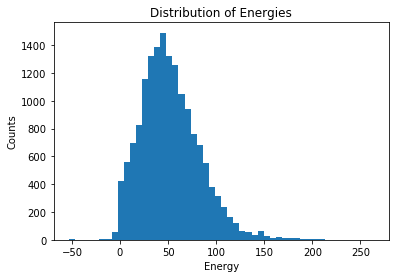
\includegraphics [scale=1.0] {img/dist.png}
  \caption{Количественное распределение энергий основного состояния молекул} 
  \label{fig:7}  
\end{figure}



В листинге \ref{ls:6} указан вывод программы при предсказании энергии основного состояния произвольных молекул из тестовой выборки. В целом, нейросеть определяет их достаточно точно.

\begin{lstlisting}[caption={Тестирование модели на небольшом списке из тестовой выборки},language=python,label={ls:6}] 
index: 851 Prediction: 0.34696415   Energy: 3.7127
index: 852 Prediction: 44.661823   Energy: 44.8169
index: 853 Prediction: 20.913294   Energy: 21.9148
index: 854 Prediction: 40.10662   Energy: 44.8035
index: 855 Prediction: 41.73383   Energy: 34.8584
\end{lstlisting}
